\documentclass[tikz,border=10pt]{standalone}
\usepackage{amsmath}
\begin{document}
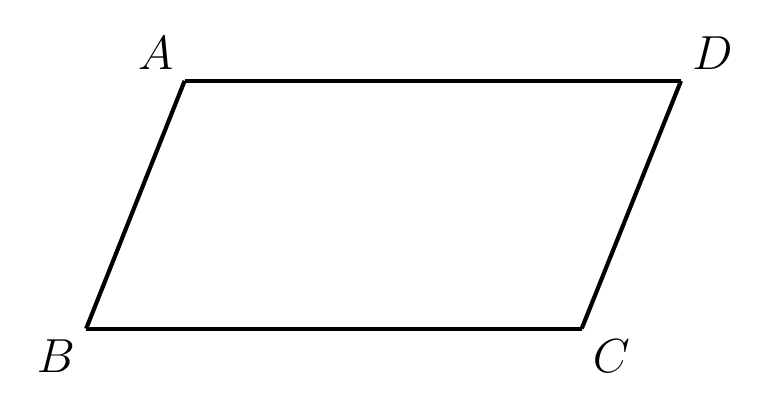
\begin{tikzpicture}[line join=round, line width=1.5pt]
\coordinate (A) at (-2.535,1.587);
\coordinate (B) at (-3.785,-1.560);
\coordinate (C) at (2.508,-1.560);
\coordinate (D) at (3.769,1.587);

  
  \draw (A) -- (D);   
  \draw (D) -- (C);   
  \draw (C) -- (B);   
  \draw (B) -- (A);   

  
  \node[above left, font=\fontsize{17}{20.4}\selectfont] at (A) {$A$};
  \node[above right, font=\fontsize{17}{20.4}\selectfont] at (D) {$D$};
  \node[below left, font=\fontsize{17}{20.4}\selectfont] at (B) {$B$};
  \node[below right, font=\fontsize{17}{20.4}\selectfont] at (C) {$C$};
\end{tikzpicture}
\end{document}